% Figure 1: architecture (hero)
\begin{figure*}[t]
  \centering
  
\includegraphics[width=0.85\textwidth]{figures/fig1_architecture.pdf}
  \caption{Deep-Dream separates navigation from factual authority. Derived concept families, observations, assertions, and graph neighborhoods form a non-authoritative overlay for scope materialization and candidate generation; the three answer paths differ in how far the answerer may go toward the verbatim sources---fused retrieval payload (rung 1), read-only memory tools (rung 2), or a sandbox of verbatim sources with verification tools and an evidence gate (rung 3). An overlay error can cause a missed scope, never a fabricated fact.}
  \label{fig:architecture}
\end{figure*}

% Figure 2: answer-path ladder (headline)
\begin{figure}[t]
  \centering
  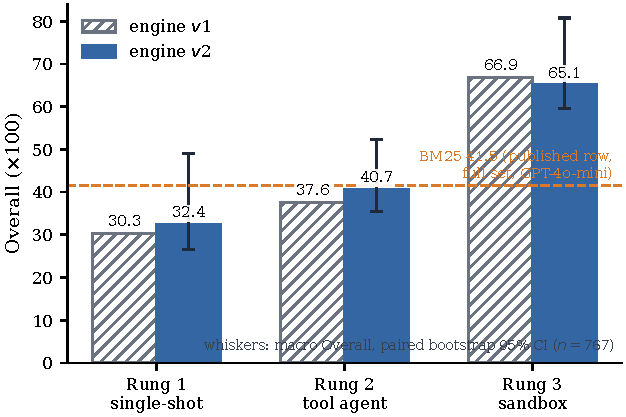
\includegraphics[width=0.9\columnwidth]{figures/fig2_ladder.pdf}
  \caption{The answer-path ladder on MemoryAgentBench (official scorer, $n{=}767$, kimi-k3 answerer, frozen libraries per generation): Overall by track for engine $v1$ (hatched) and $v2$ (solid); whiskers, shown on the $v2$ bars only, are paired-bootstrap 95\% CIs over the 767 shared questions. The BM25 row (41.5, official paper, full set, GPT-4o-mini) is drawn as a published-reference band, not a same-protocol bar: answerer, judge, and subset differ; no subtraction is implied.}
  \label{fig:ladder}
\end{figure}
